%%%%%%%%%%%%%%%%%%%%%%%%%%%%%%%%%%%%%%%%%%%%%%%%%%%%%%
%%%%%%%%%% Configurações Iniciais E Pacotes %%%%%%%%%%
%%%%%%%%%%%%%%%%%%%%%%%%%%%%%%%%%%%%%%%%%%%%%%%%%%%%%%


\documentclass[12pt]{article}

% Codificação e idioma
\usepackage[utf8]{inputenc}   % Permite acentuação
\usepackage[T1]{fontenc}      % Melhora a saída da fonte
\usepackage[brazil]{babel}    % Ajuste para pt-br

% Layout e fontes
\usepackage{geometry}               % Margens personalizadas
\usepackage{newtxtext,newtxmath}    % Fonte Times New Roman para texto e matemática
\usepackage{setspace}               % Controle de espaçamento entre linhas
\usepackage{indentfirst}            % Primeiro parágrafo de cada seção será indentado automaticamente
\usepackage{eso-pic}                % Adiciona variados elementos na página

% Tabelas e gráficos
\usepackage{booktabs}        % Tabelas bonitas
\usepackage{graphicx}        % Inclusão de imagens

% URLs e links personalizados
\usepackage[colorlinks=true,
            linkcolor=cyan!30!blue,
            citecolor=cyan!30!blue,
            urlcolor=cyan!30!blue
            pdfauthor={Rafael Gomes Carneiro},
            pdftitle={Relatório Cíentifico - Bitcoin: A História em Dados}]{hyperref}
            
\usepackage[capitalize,nameinlink]{cleveref}  
% capitalize: coloca a primeira letra maiúscula em "Figura", "Tabela", etc
% nameinlink: Deixa o nome da referência também como link (não só o número)

% Configura os links
\crefname{figure}{Figura}{Figuras}

%Ajuste de margens das páginas 
\geometry{
  a4paper,
  top=3cm,
  left=3cm,
  bottom=2cm,
  right=2cm
}

%%%%%%%%%%%%%%%%%%%%%%%%%%%%%%%%%%%%%%%%%%%%%%%%%%%%%%

\title{Bitcoin: A História em Dados}
\author{Bruce Trevisan \\ 
        Nicolas Palombo Lucas \\ 
        Otávio Ribeiro Mello \\ 
        Rafael Gomes Carneiro}
\date{ME115B - Linguagem R \\ 
        Tatiana Andrea Benaglia Carvalho \\ 
        Campinas, 2025}

%%%%%%%%%%%%%%%%%%%%%%%%%%%%%%%%%%%%%%%%%%%%%%%%%%%%%%

\begin{document}

\pagenumbering{gobble}

% Página de capa separada
\AddToShipoutPictureBG*{
    
\includegraphics[width=\paperwidth,height=\paperheight]{Imagens/Fundo.png}
}
% Plano de fundo

\begin{titlepage}
    \centering
    \vspace*{2.5cm}
    
    {\Huge \bfseries Bitcoin: \\ A História em Dados \par}
    
    \vspace{2cm}

    \begin{figure} [h]
        \centering
        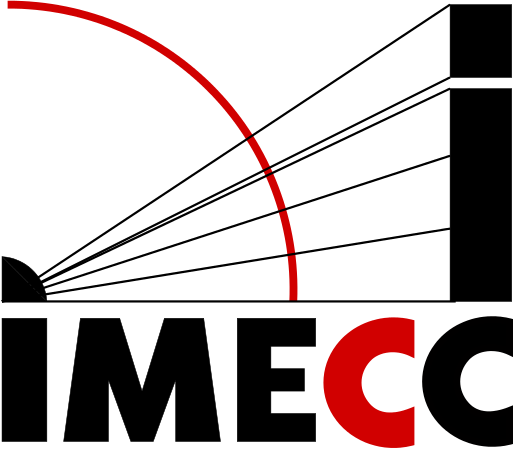
\includegraphics[width=0.3\linewidth]{Imagens/imecc-logo.png}
    \end{figure}

    { 
        {\large Autores: \par}
        {\large Bruce Trevisan \par}
        {\large Nicolas Palombo Lucas \par}
        {\large Otávio Ribeiro Mello \par}
        {\large Rafael Gomes Carneiro \par}
    }
    
    \vfill
    {\large ME115B - Linguagem R \par}
    {\large Tatiana Andrea Benaglia Carvalho \par}
    {\large Campinas, 2025 \par}
    
    
\end{titlepage}

\clearpage

\tableofcontents



\newpage

\section{\textbf{Resumo}}

TESXTE TEXTE 



TEXETE 
 TET EVBRVM
 VRTBVRTBMOIT
 BERI NIN
 VRTOVIN

 OIVORNN R
 OINROINRJ P
 OINORT O



 VTRVOT VOR OI


 \cref{fig:Candle Graph}

\newpage

\pagenumbering{arabic} % Começo de contagem de folhas

\section{\textbf{Introdução}}

\subsection{\textbf{O que são criptomoedas?}}

Por definição, criptomoedas são qualquer tipo de moeda digital ou virtual que utiliza criptografia para garantir a realização de transações. Elas não têm autoridade central de emissão e sem regulação. Em contrapartida, elas utilizam um sistema de criptografia chamado de blockchain, além de outros sistemas de criptografia descentralizados para registrar transações e emitir novas unidades. 
\textbf{Blockchain é um banco de dados distribuído que consegue fazer um} compartilhamento de informações dentro de uma rede. Essas informações podem ser variadas, agrupadas em bloco a partir de criptografia, de uma forma que consiga trazer consigo o histórico completo e imutável das transações anteriores. Garantindo uma rede de operações concisas, seguras e confiáveis para qualquer um que desejar entrar nessa rede.

As criptomoedas atuam com diversas funções e objetivos além de um simples meio de transação monetária para uso diário. Elas podem ser reserva de valores; atuação como \textbf{ações de investimento}, por conta de sua alta volatilidade de seu valor; descontos em taxas; garantia de algum serviço; entre muitas outras funções.

Um dos maiores exemplos de criptomoedas são o Bitcoin e o Ether. O \textit{Ether} valendo cerca de \textbf{2.55 mil dólares americanos}, além do \textit{Bitcoin}, tendo mais de \textbf{100 mil dólares americanos} e sendo a criptomoeda mais famosa do mundo.

\subsection{\textbf{O que é \textit{Bitcoin}?}}
Lançado em 2008, com o pseudônimo de Satoshi Nakamoto, uma nova ideia foi criada e posta ao mundo, com a criação do Bitcoin. O Bitcoin é atualmente a criptomoeda mais famosa do mundo, além de ser a mais valorizada atualmente, ultrapassando a marca de US\$100.000,00 

Devido ao fato do Bitcoin ser uma criptomoeda, logo, ela não tem uma emissão regularizada e centralizada, a emissão de novas moedas no mercado é de uma outra forma. É usado o termo "mineração". Esse processo consiste na resolução de quebra-cabeças matemáticos complexos feitos por hardware e software especializados para a mineração de Bitcoin. A mineração não é exclusiva de um grupo de pessoas, empresas ou bancos. Contanto que tenha energia e um hardware de mineração, é possível obter um bloco de Bitcoin.

Os blocos de Bitcoin são os produtos e agrupamentos de transações individuais dos últimos dez minutos de cada mineração. Cada bloco é único e fechado, cada um criando seu próprio número \textit{Hash}, que é onde estão codificadas as transações. Cada novo bloco precisa ter em seu conteúdo as informações do bloco anterior, o que garante uma veracidade de que não será manipulado ou alterado. Cada bloco gerado é equivalente a uma quantidade específica de Bitcoin, cada bloco tem atualmente 3.125 BTC (Bitcoin).

Com tal unicidade, garante uma individualidade perante cada unidade de moeda não seja possuída por mais de um portador. O que torna a concorrência de cada máquina para garantir seu bloco próprio maior ainda, incentivando cada vez mais a melhora dos computadores para fazer a mineração. Além disso, para a autenticação no sistema de Prova de Trabalho (PoW) do Bitcoin, os computadores de mineração precisam comprovar a energia gasta para a mineração de cada bloco. O que reforça a segurança e autenticidade de cada máquina e bloco minerado.

% Gráfico Principal
\begin{figure}
    \centering
    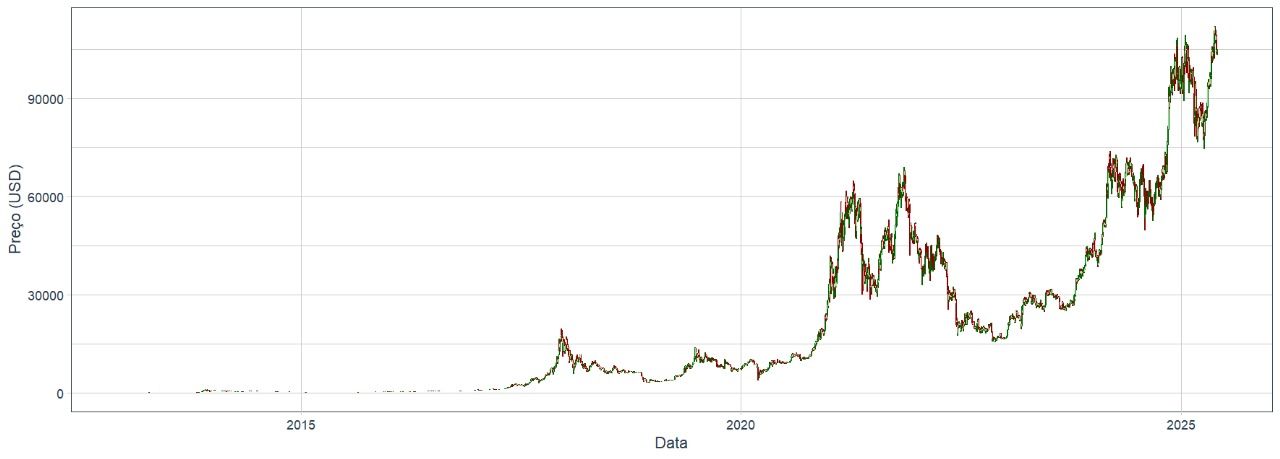
\includegraphics[width=1\linewidth]{Imagens/Grafico-Princial.jpg}
    \caption{Histórico do Valor do Bitcoin}
    \label{fig:Candle Graph}
\end{figure}

\subsection{\textbf{Eventos Importantes:}}

A lei da oferta e demanda tem grande influencia sobre a valorização e  desvalorização do Bitcoin.  Assim como nos mercados tradicionais, quando a oferta de um produto é limitada e sua demanda aumenta, o seu valor tende a aumentar também. Só que no casso do Bitcoin, ele é tanto o produto quanto uma possível moeda de troca externa. Isso tudo é realçado por ter uma oferta limitada à no máximo 21 milhões de unidades. No entanto, também existe outros fatores que pode influenciar  em seu valor, tendo os principais exemplos: o evento Halving, o caso da Mt. Gox e a pandemia  de COVID-19.

Ocorrendo aproximadamente a cada 4 anos, o evento Halving  reduz pela metade o ganho de Bitcoin por bloco minerado, diminuindo a entrada de novos bitcoins no mercado. Este evento é associado geralmente com a valorização do bitcoin, já que aumenta a escassez da moeda, favorecendo a sua valorização.

Acontecimentos externos também podem ocasionar a desvalorização da moeda, como por exemplo a falência da empresa Mt. Gox, em 2014. Na época, a maior corretora de criptomoedas do mundo, acabou perdendo por volta de 800 mil bitcoins após sofrer uma sequência de invasões cibernéticas. Causando uma queda brusca no valor do bitcoin e afetando a confiança neste mercado.

A pandemia de COVID-19 em 2020 também teve um grande impacto no valor do bitcoin. Com a incerteza global ao início da pandemia, o Bitcoin apresentou uma queda em seu valor, porém com a desvalorização das moedas fiduciárias, a bitcoin passou a ser procurada como investimento alternativo, resultando em uma significativa valorização.

\newpage

\section{\textbf{Material e Métodos:}}

\subsection{\textbf{Eventos Importantes:}}

\subsubsection{\textbf{O que é o Evento \textit{Halving}?}}
O evento Halving é um acontecimento periódico em que o número de Bitcoins em cada bloco minerado é reduzido pela metade, ocorre especificamente a cada 210 mil blocos minerados. Apesar de sua data não ser totalmente certa, é possível estimar com grande precisão, normalmente ocorrendo a cada 4 anos.

Seu objetivo é tentar controlar o valor da moeda com a inflação. O Halving não possui relações diretas no desejo de aumentar diretamente o valor de mercado da moeda, suas intenções valem tentativa de controle sobre o valor da moeda com a inflação. Adicionando o fato de que seu(s) criador(es) já deixaram bem explícito que haverá uma quantidade limitada de unidades de Bitcoin, o que já está fixo na quantidade de 21 milhões.

Os efeitos do halving influenciam em seu valor indiretamente, já que pela lei da oferta e demanda, com a queda da oferta sobre o Bitcoin e que normalmente há um aumento na demanda, seu preço aumenta.

Ele já ocorreu 4 vezes. Em 2012, 2016, 2020 e 2024.

% Tabela da Linha do Bitcoin Halving 
\begin{figure}[h]
    \centering
    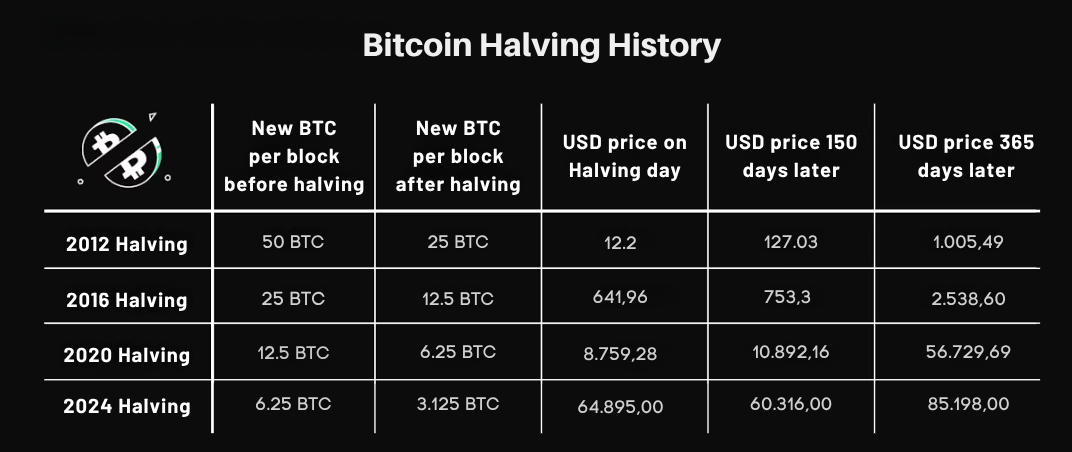
\includegraphics[width=0.8\textwidth]{Imagens/Tabela_Halving.png}
    \caption{Tabela Cronológica do Evento Halving}
    \label{fig:Tabela Cronologica do Evento Halving}
\end{figure}

\subsubsection{\textbf{A Queda da Mt. Gox}}
Em 2006, a empresa \textit{Magic: The Gathering Online Exchange}, ou mais conhecida por somente \textbf{Mt. Gox}, fora criada por Jed McCaleb com o objetivo de ter uma plataforma de troca de cartas de \textit{Magic: The Gathering Online}, um jogo online famoso na época.  Porém, em 2010, começou a entrar no ramo de mineração de Bitcoin. Porém, com a venda ao francês Mark Karpelès, em 2011 e adotando sua sede no Japão, ela se tornou uma corretora de criptomoedas, explorando a crescente popularidade das criptomoedas.

Rapidamente tornando-se a maior corretora no mercado emergente das criptomoedas. Conseguindo ter a maior bolsa de valores sobre o Bitcoin no Mundo inteiro. Em seu auge — no ano de 2013 — ela administrava mais de 70\% das transações em Bitcoin no mundo. Porém, o seu colapso no ano seguinte trouxe à tona um grande alerta sobre a segurança e a falta de regulamentação no mercado de Criptomoedas.

Em 07 fevereiro de 2014, a corretora alegou problemas técnicos e suspendeu os saques de Bitcoin. Em 24 de fevereiro ocorreu Fechamento da Exchange — a plataforma de transação de Criptomoedas, e logo em seguida, em 28 de Fevereiro, a Mt. Gox declarou falência. Expondo uma perda de cerca de 850 mil Bitcoins — Aproximadamente 450 milhões de dólares na época — O que representava cerca de 6\% de todo a volume de Bitcoins em circulação no momento. Essa perda provocou uma queda no valor do Bitcoin em quase 36\% no período de ferreiro e março do mesmo ano. 

% Gráfico sobre o Impacto da Mt. Gox
\begin{figure}
    \centering
    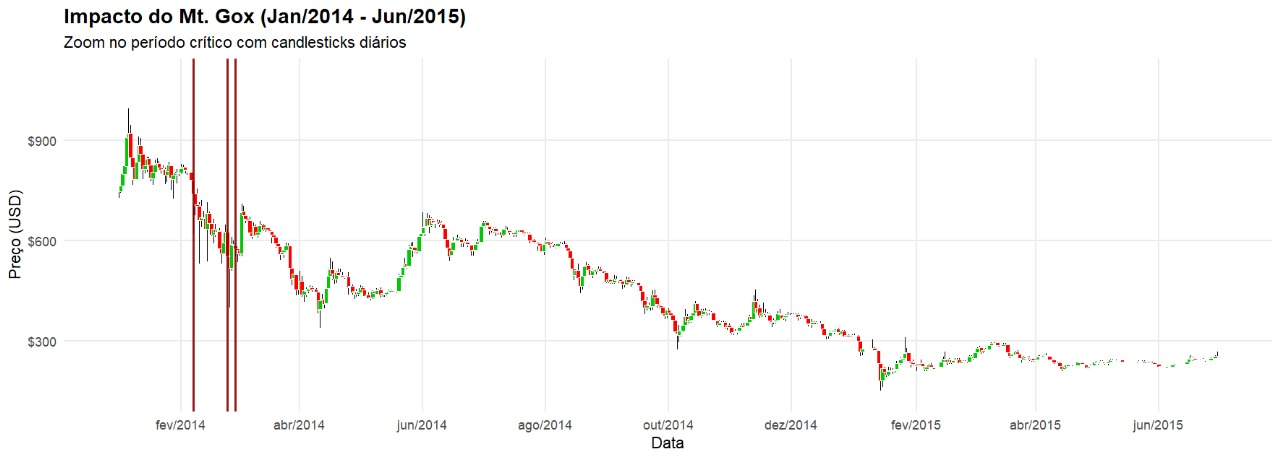
\includegraphics[width=1\textwidth]{Imagens/Mt_Gox_Grafico.jpg}
    \caption{Impacto da Mt. Gox}
    \label{fig:Mt. Gox Gráfico}
\end{figure}

Posteriormente, a empresa encontrou 200 mil Bitcoins (dos 850 mil perdidos) em carteiras frias — dispositivos offline para armazenamento seguro, porém a perda total ainda permanece como um dos maiores desastres financeiros no ramo das criptomoedas.

O motivo dessa perda pela empresa forem vindos de uma má gestão da plataforma, agravada por falhas no sistema de segurança. Acredita-se que hackers de origem russa foram retirando Bitcoins de forma gradual, explorando vulnerabilidades no sistema da corretora. A falta de controle das carteiras digitais e a falha nos mecanismos de transações e saques — que não detectaram ações irregulares, foram só exemplos de erros que tinham em seus sistema.

A quebra da Mt. Gox abalou  significativamente a comunidade Bitcoin. Comprometendo a credibilidade nas corretoras de criptomoedas, impactando esse mercado que ficou cravado no público por anos. Esse episódio foi um alerta indesejado sobre a vulnerabilidade que tinha nesse mercado,  evidenciando a necessidade de fortalecimento de práticas de regulação para proteger os investidores para reatar a confiança no mercado cripto.

\subsubsection{\textbf{Pandemia COVID-19}}

No começo da pandemia de COVID-19, houve um caos generalizado junto com uma transformação abrupta do cotidiano. Nenhum setor foi isento e não teve alterações, incluindo naturalmente, o ramo financeiro de criptomoedas. Assim como as moedas estatais e tradicionais, o Bitcoin também foi afetado e teve uma desvalorização de até 50\% de seu valor, devido a grande incerteza econômica global. Entretanto, com os governos aumentando aa emissão de moedas fiduciárias, o Bitcoin se fortaleceu como um ativo de proteção contra inflação, conseguindo recuperar e alcançar seu preço máximo em 2021, ou pelo até o ano de 2024, que teve mais uma grande serie de aumento de seu valor.

% Gráfico Pandemia

\begin{figure}
    \centering
    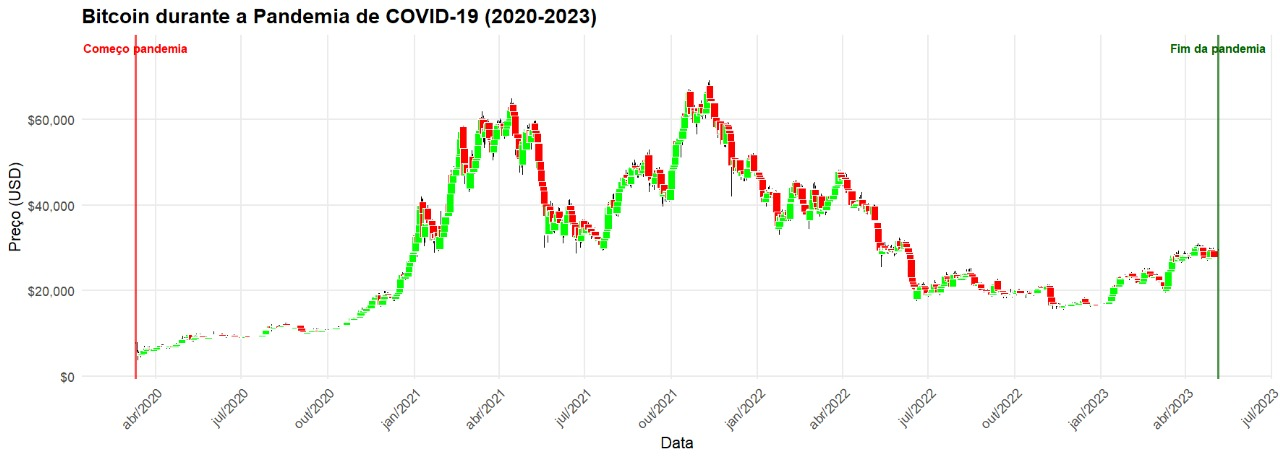
\includegraphics[width=0.8\textwidth]{Imagens/grafico_pandemia.jpg}
    \caption{Bitcoin na Pandemia}
    \label{fig:pandemia}
\end{figure}

Vemos na \cref{fig:Candle Graph}, que logo no começo de 2020 temos um crescimento no valor de moeda do Bitcoin, devido ao pré-Halving. Assim como foi previsto, em 11 de maio aconteceu o evento halving. Porém, vemos também uma queda logo em seguida, representando a queda na economia global. Porém, pouco tempo depois já houve uma crescente em seu valor, representando na indução de um ativo contra a inflação.

Essa serie de aumento e redução de preços são variadas. Como falado, a desvalorização se deve a crise financeira mundial em conjunto com a pandemia COVID-19. Porém, sua valorização é mais devido à percepção de uma forma de proteção e diversificação para empresas e pessoas ainda conseguirem um meio viável de continuar com transações cotidianas. Por conta disso, a utilização de criptomoedas foi ampliado, entrando no cotidiano a fundo dessa vez. A integração de criptomoedas na forma de pagamento impactou o mundo, além de impulsionar o valor do Bitcoin.

Apesar de sua alta com o grande aumento do seu valor, o bitcoin acabou consolidando-se como “ouro digital”, ganhando destaque como um dos principais investimentos alternativos no mercado financeiro.

\subsection{\textbf{Material utilizado:}}

O banco de dados, “Bitcoin Historical Data”, que fora extraído da plataforma Kaggle, armazena todos os dados da história do Bitcoin em intervalos de 1 minuto, extraídos de Exchange de Bitcoin — plataformas de transações específicas para criptomoedas — onde as negociações ocorrem.	

O arquivo está no formato \texttt{.csv}, apresentando 6 colunas com variáveis numéricas em formato decimal, sendo separadas por ponto. O tamanho do arquivo é de 369.29 MB. Cobrindo o período de 1 de janeiro de 2012 até o presente, recebendo atualizações diárias para inclusão de novos dados. Entretanto, para a análise dos dados, o banco de dados será restringido até a  data de 01 de Junho de 2025.

\subsubsection{\textbf{As principais variáveis:}}

\begin{itemize}
    \item \textbf{Timestamp}: Indica a hora de início do tempo de 60 segundos, no horário Unix — tempo em segundos desde 1 de janeiro de 1970.
    \item \textbf{Open, High, Low e Close}: mostram como o preço se comportou no período de um minuto:
    \begin{itemize}
        \item \textbf{Open}: Preço de abertura na janela de tempo inicial.
        \item \textbf{High}: Preço mais alto na janela de 1 minuto.
        \item \textbf{Low}: Preço mais baixo na janela de 1 minuto.
        \item \textbf{Close}: Preço no fechamento da janela de tempo inicial.
    \end{itemize}
    \item \textbf{Volume}: Volume de BTC negociados nesta janela de tempo.
\end{itemize}

\subsection{\textbf{Metodologia:}}

A análise foi realizada na linguagem \texttt{R}, versão \texttt{4.5.0}, utilizando diversos pacotes para a manipulação e visualização dos dados. No dataset, os dados são distribuídos em intervalos de 1 minuto, porém para facilitar a análise, os dados foram agrupados por dia — mas sem alterar o seu conteúdo, para melhor visualização nos gráficos.

Para a limpeza e manipulação das amostras, foram utilizados os pacotes \texttt{tidyverse}, \texttt{magrittr}, \texttt{tidyquant} e \texttt{lubridate}. O \texttt{tidyverse} inclui o \texttt{dplyr}, utilizado para filtragem e agrupamento dos dados; o \texttt{lubridate} foi empregado para a conversão do timestamp; enquanto \texttt{magrittr} e \texttt{tidyquant} foram usados para facilitar a manipulação e as análises financeiras dos dados.

Para a criação dos gráficos foi utilizado o \texttt{ggplot2}, \texttt{tidyquant} e \texttt{scales}, para a elaboração de \textit{candlesticks} e linhas, que auxiliam a interpretação do comportamento do preço do Bitcoin. Além disso, para alguns cálculos financeiros e análise de desempenho, foram utilizados os pacotes \texttt{quantmod}, \texttt{TTR} e \texttt{PerformanceAnalytics}.

Fora criado gráficos de candlestick  para melhor visualização do historico de valor do Bitcoin ao decorrer dos anos. Focando tanto em eventos específicos, como a queda da Mt. Gox, quanto ampliando para o período completo para melhor noção geral. Além de utilizar gráficos de dispersão para analises de correlação e melhor discernimento do comportamento humano em relação ao Bitcoin.




\newpage % Limpar visualmente no pdf.


\section{\textbf{Resultados:}}

\subsection{\textbf{Analisando Gráficos:}}

Os dados mostram padrões interessantes. Nós anos de Halving, vemos sempre uma valorização no logo após o começo dos anos, um acontecimento conhecido como "pre-halving uptrend", ou em português, "Tendência de alta pré-Halving". O que mostra uma valorização pouco meses antes do previsto do Evento Halving realmente acontecer. 

Vemos na \cref{fig:Candle Graph} muito bem as tendências de valorização. É possível visualizar melhor devido as proporções  maiores nos anos de 2020 e de 2024. Contudo podemos aplicar para mais eventos.

\begin{figure}[h]
    \centering
    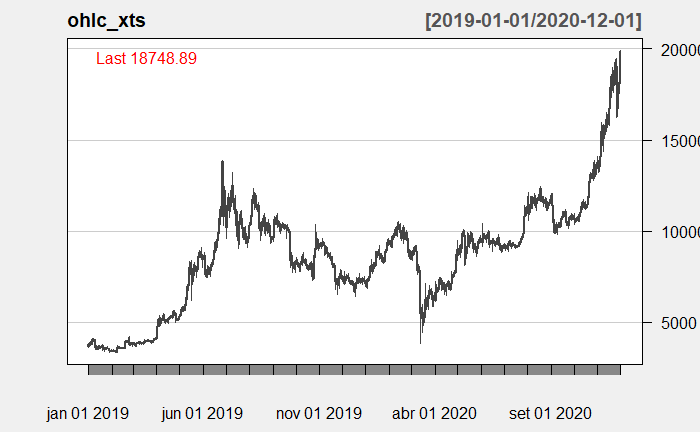
\includegraphics[width=0.8\linewidth]{Imagens/Grafico_rascunho_pre.png}
    \caption{Rascunho do Gráfico Pré Pandemia}
    \label{fig:pre pandemia}
\end{figure}

% PRETENDO TIRAR ESSE GRÁFICO DEPOIS
% REFERENCIA CITADA --> MUDAR PARA O GRAFICO PRINCIPAL DO COMEÇO. APROVEITAR QUE TEM "LINK DIRETO"
% EU POSSO PEDIR PARA O NICOLAS EXPANDIR O GRÁFICO DA PANDEMIA PARA UM POUCO DO PRE-PENDEMIA.

Vindo de antes da Pandemia do COVID-19, em meados de janeiro de 2019, que a popularidade do Bitcoin não estava muito boa. Começou a crescer perto de junho, devido também a outros fatores também, mas principalmente por conta da euforia da pré-Halving. O seu valor de mercado permaneceu com valores instáveis, valorizando e desvalorizando com irregularidade. 

É perceptível uma queda brusca em abril de 2020 devido a pandemia COVID-19, mas isso não se perdurou por muito tempo, voltando ao seu valor habitual poucos meses depois. Entretanto, como podemos ver na \cref{fig:pandemia}, o seu maior crescimento foi quando se aproximava de 2021, que foi o começo da onda de percepção do Bitcoin como um ativo seguro contra a inflação.

\subsection{\textbf{Análise dos Testes de Correlação}}

% Gráficos de correlação
\begin{figure}[ht]
  \centering
  \begin{minipage}{0.48\linewidth}
    \centering
    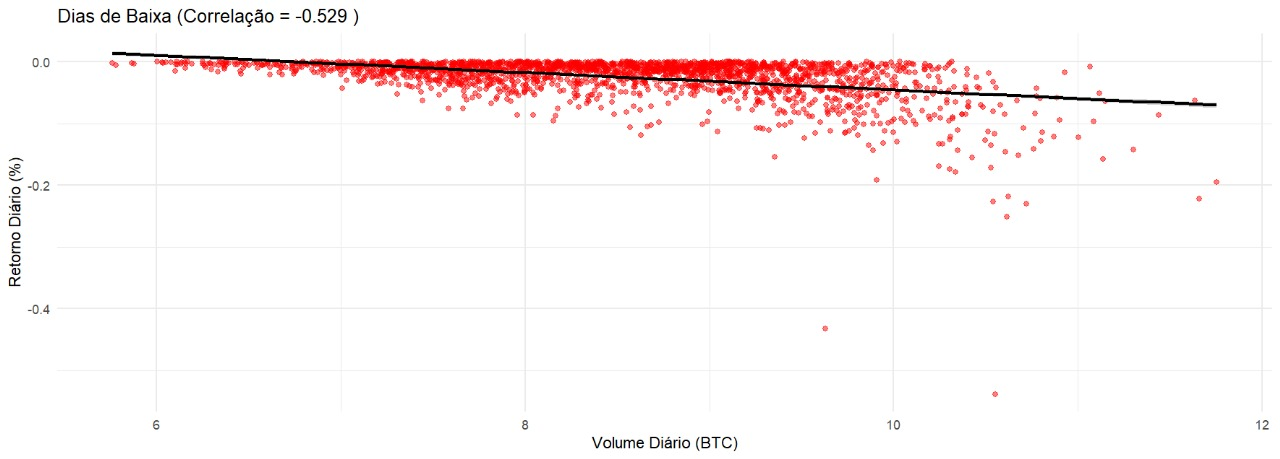
\includegraphics[width=\linewidth]{Imagens/Correlacao Negativa.jpg}
    \caption{Gráfico de Correlação Negativa}
    \label{fig:correlacao-negativa}
  \end{minipage}\hfill
  \begin{minipage}{0.48\linewidth}
    \centering
    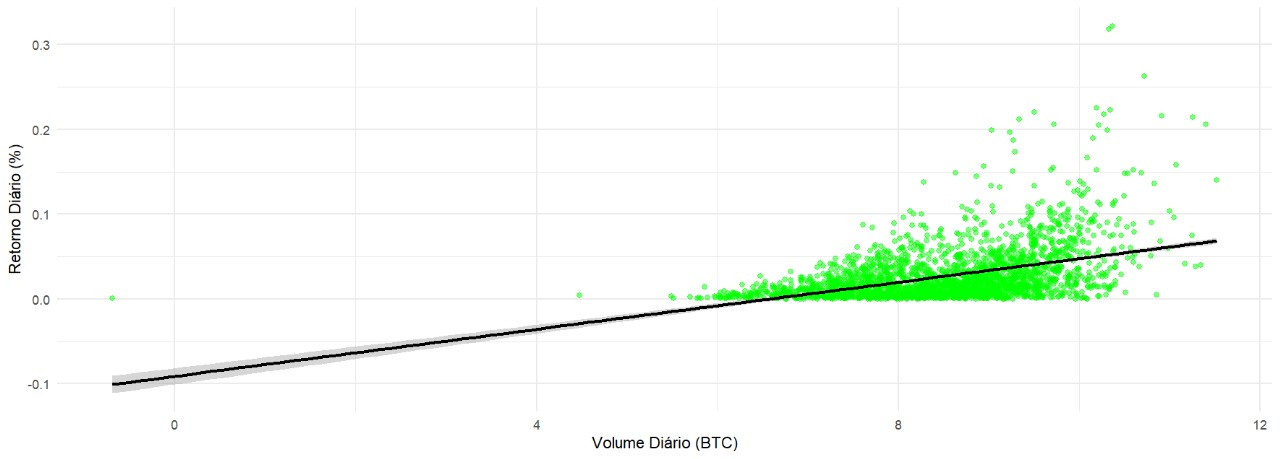
\includegraphics[width=\linewidth]{Imagens/Correlacao Positiva.jpg}
    \caption{Gráfico de Correlação Positiva}
    \label{fig:correlacao-positiva}
  \end{minipage}
\end{figure}

Definiremos as hipóteses para 


\subsubsection{Definição das Hipóteses}
\begin{itemize}
  \item \textbf{Hipótese nula (H$_0$):} $\rho = 0$ — Sem correlação linear entre retorno diário e volume.
  \item \textbf{Hipótese alternativa (H$_A$):} $\rho \neq 0$ — Há uma correlação linear entre retorno diário e volume.
\end{itemize}

\subsubsection{Dias de Alta}
\begin{itemize}
  \item \textbf{Coeficiente de correlação (r):} $0,493$  
    Indica correlação moderadamente positiva entre retorno e volume em dias de valorização.
  \item \textbf{Estatística $t$:} $t = 27{,}902$ com 2\,421 graus de liberdade.  
    Valor elevado reforça a evidência \textbf{contra H$_0$}.
  \item \textbf{p-valor:} $p < 2{,}2\times10^{-16}$  
    Praticamente zero — altamente significativo. Rejeitamos H$_0$.
  \item \textbf{Intervalo de confiança 95\%:} $[0,463,\;0,523]$  
    Com 95\% de confiança, a correlação verdadeira está neste intervalo.
\end{itemize}

\paragraph{Interpretação.}
Em dias de alta, volume e retorno crescem juntos, sugerindo que movimentos de valorização atraem maior interesse comprador.

\subsubsection{Dias de Baixa}
\begin{itemize}
  \item \textbf{Coeficiente de correlação (r):} $-0,529$  
    Indica correlação moderadamente negativa entre retorno e volume em dias de desvalorização.
  \item \textbf{Estatística t:} $t = -28{,}574$ com 2\,102 graus de liberdade.  
    Magnitude elevada (sinal negativo indica direção inversa) reforça evidência contra H$_0$.
  \item \textbf{p-valor:} $p < 2{,}2\times10^{-16}$  
    Altamente significativo — rejeitamos H$_0$.
  \item \textbf{Intervalo de confiança 95\%:} $[-0,559,\;-0,497]$  
    Com 95\% de confiança, a correlação populacional verdadeira é negativa e está neste intervalo.
\end{itemize}

\paragraph{Interpretação.}
Em dias de baixa, o aumento de volume acompanha quedas de preço, caracterizando vendas em pânico ou liquidações forçadas.

\subsubsection{Considerações Finais}
Os resultados mostram uma assimetria de mercado:
\begin{itemize}
  \item Em \emph{alta}, maior volume ocorre junto a retornos positivos (pressão compradora).
  \item Em \emph{baixa}, maior volume ocorre junto a retornos negativos (vendas aceleradas).
\end{itemize}
Esse padrão assimétrico é relevante para modelagem de risco e elaboração de estratégias de portfólio.


\newpage

\section{\textbf{Considerações Finais:}}



\newpage

\section{\textbf{Referências:}}

% Colocando referências
\renewcommand{\refname}{}  % Tira o Título "Referências" do 'thebibliography'
\vspace*{-1.5cm}           % Remove o espaço antes

\begin{thebibliography}{99}
\sloppy

    \bibitem{ref1} VRANKEN, Harald. Sustainability of bitcoin and blockchains. Current Opinion in Environmental Sustainability, [S.l.], v. 28, p. 1-9, 2017. Disponível em: 
    \href{https://www.sciencedirect.com/science/article/pii/S1877343517300015}{https://www.sciencedirect.com/science/article/pii/S1877343517300015}.
    Acesso em: 4 jun. 2025.
    
    \bibitem{ref2} REDAÇÃO NUBANK. O que é bitcoin e como funciona essa moeda virtual? Nubank, 11 mar. 2020. Atualizado em: 11 out. 2024. Disponível em: 
    \href{https://blog.nubank.com.br/o-que-e-bitcoin/}{https://blog.nubank.com.br/o-que-e-bitcoin/}.
    Acesso em: 4 jun. 2025.
    
    \bibitem{ref3} BBC NEWS BRASIL. Bitcoin: o que explica sobe e desce da criptomoeda, com queda vertiginosa após valorização recorde? [S.l.], 26 maio 2021. Disponível em: 
    \href{https://www.bbc.com/portuguese/internacional-57238550}{https://www.bbc.com/portuguese/internacional-57238550}.
    Acesso em: 4 jun. 2025.
    
    \bibitem{ref4} KASPERSKY. O que é criptomoeda e como funciona? [S.l.]: Kaspersky. Disponível em: 
    \href{https://www.kaspersky.com.br/resource-center/definitions/what-is-cryptocurrency}{https://www.kaspersky.com.br/resource-center/definitions/what-is-cryptocurrency}. 
    Acesso em: 4 jun. 2025.
    
    \bibitem{ref5} BTG PACTUAL. Ativos financeiros: o que são, principais ativos e como escolher. [S.l.], 4 out. 2024. Disponível em:
    \href{https://content.btgpactual.com/blog/conceitos-basicos/ativos-financeiros-o-que-sao-principais-ativos-e-como-escolher}{https://content.btgpactual.com/blog/conceitos-basicos/ativos-financeiros-o-que-sao-principais-ativos-e-como-escolher}.
    Acesso em: 4 jun. 2025.
    
    \bibitem{ref6} BTG PACTUAL. Entenda o que são Criptomoedas e qual a sua utilidade. [S.l.],  28 out. 2023. Disponível em: 
    \href{https://content.btgpactual.com/blog/criptomoedas/entenda-o-que-sao-criptomoedas-e-qual-a-sua-utilidade}{https://content.btgpactual.com/blog/criptomoedas/entenda-o-que-sao-criptomoedas-e-qual-a-sua-utilidade}. 
    Acesso em: 4 jun. 2025.
    
    \bibitem{ref7} INFOMONEY. O que é o halving do Bitcoin? [S.l.], [S.l.], 4 mar. 2024. Disponível em: 
    \href{https://www.infomoney.com.br/guias/halving-do-bitcoin/}{https://www.infomoney.com.br/guias/halving-do-bitcoin/}. 
    Acesso em: 4 jun. 2025.
    
    \bibitem{ref8} BITPANDA. What is a Bitcoin halving and what happens on the network? [S.l.]. Disponível em: 
    \href{https://www.bitpanda.com/academy/en/lessons/what-is-a-bitcoin-halving-and-what-happens-on-the-network/}{https://www.bitpanda.com/academy/en/lessons/what-is-a-bitcoin-halving-and-what-happens-on-the-network/}. 
    Acesso em: 4 jun. 2025.
    
    \bibitem{ref9} GRATTON, Peter. What is a block in the crypto blockchain, and how does it work? [S.l.], 21 jan. 2025. Disponível em: 
    \href{https://www.investopedia.com/terms/b/block-bitcoin-block.asp}{https://www.investopedia.com/terms/b/block-bitcoin-block.asp}. 
    Acesso em: 4 jun. 2025.
    
    \bibitem{ref10} CRYPTOPEDIA STAFF. How a Block in the Bitcoin Blockchain Works. [S.l.], 2022. Disponível em: 
    \href{https://www.gemini.com/pt-BR/cryptopedia/what-is-block-in-blockchain-bitcoin-block-size}{https://www.gemini.com/pt-BR/cryptopedia/what-is-block-in-blockchain-bitcoin-block-size}.  
    Acesso em: 4 jun. 2025.
    
    \bibitem{ref11} THE INVESTOPEDIA TEAM. What Was Mt. Gox? Definition, History, Collapse, and Future. [S.l.], 23 abr. 2024. Disponível em: 
    \href{https://www.investopedia.com/terms/m/mt-gox.asp}{https://www.investopedia.com/terms/m/mt-gox.asp}. 
    Acesso em: 4 jun. 2025.
    
    \bibitem{ref12} GREGO, Maurício. Roubo de US\$ 388 milhões em bitcoins leva Mt. Gox a fechar. São Paulo, 25 fev. 2014. Disponível em: 
    \href{https://exame.com/tecnologia/roubo-de-us-388-milhoes-em-bitcoins-leva-mt-gox-a-fechar/}{https://exame.com/tecnologia/roubo-de-us-388-milhoes-em-bitcoins-leva-mt-gox-a-fechar/}.
    Acesso em: 4 jun. 2025.
    
    \bibitem{ref13} POLLOCK, Darryn. O desastre que foi Mt. Gox: quatro anos depois. [S.l.], 9 mar. 2018. Disponível em: 
    \href{https://br.cointelegraph.com/news/the-mess-that-was-mt-gox-four-years-on}{https://br.cointelegraph.com/news/the-mess-that-was-mt-gox-four-years-on}. 
    Acesso em: 4 jun. 2025.
    
    \bibitem{ref14} BBC NEWS BRASIL. Como o Bitcoin atingiu valor recorde em meio à pandemia. [S.l.], 17 dez. 2020. Disponível em: 
    \href{https://www.bbc.com/portuguese/geral-55349371}{https://www.bbc.com/portuguese/geral-55349371}. 
    Acesso em: 4 jun. 2025.
    
    \bibitem{ref15} JUARROS, Santiago. Como o ano de 2020 afetou o mercado cripto? [S.l.], 27 jan. 2021. Disponível em: 
    \href{https://launchpad-br.ripio.com/blog/como-o-ano-de-2020-afetou-o-mercado-cripto}{https://launchpad-br.ripio.com/blog/como-o-ano-de-2020-afetou-o-mercado-cripto}. 
    Acesso em: 4 jun. 2025.
    
    \bibitem{ref16} TRUST WALLET. The story of Mt. Gox: Explained. [S.l.], 17 jul. 2024. Disponível em: 
    \href{https://trustwallet.com/blog/cryptocurrency/mt-gox-explained}{https://trustwallet.com/blog/cryptocurrency/mt-gox-explained}. 
    Acesso em: 4 jun. 2025.
    
    \bibitem{ref17} WICKHAM, Hadley. Easily Install and Load the 'Tidyverse' (versão 2.0.0). Vienna: R Foundation for Statistical Computing, 22 fev. 2023. [pacote de computador]. Disponível em: 
    \href{https://tidyverse.tidyverse.org}{https://tidyverse.tidyverse.org}. 
    Acesso em: 14 jun. 2025.
    
    \bibitem{ref18} DANCHO, Matt; VAUGHAN, Davis. Tidy quantitative financial analysis (versão 1.0.11). Vienna: R Foundation for Statistical Computing, 13 fev. 2025. [Pacote de computador]. Disponível em: 
    \href{https://business-science.github.io/tidyquant/}{https://business-science.github.io/tidyquant/}. 
    Acesso em: 14 jun. 2025.
    
    \bibitem{ref19} WICKHAM, Hadley et al. Create elegant data visualisations using the grammar of graphics (versão 3.5.2). [S.l.]: R Foundation for Statistical Computing, 9 abr. 2025. [Pacote de computador]. Disponível em: 
    \href{https://ggplot2.tidyverse.org}{https://ggplot2.tidyverse.org}. 
    Acesso em: 14 jun. 2025.
    
    \bibitem{ref20} RYAN, Jeffrey A. Quantitative financial modelling framework (versão 0.4.27). [S.l.]: R Foundation for Statistical Computing, 6 abr. 2025. [Pacote de computador]. Disponível em: 
    \href{https://www.quantmod.com}{https://www.quantmod.com}. 
    Acesso em: 14 jun. 2025.
    
    \bibitem{ref21} ULRICH, Joshua; SMITH, Ethan B. Technical trading rules (versão 0.24.4). [S.l.]: R Foundation for Statistical Computing, 28 nov. 2023. [Pacote de computador]. Disponível em: 
    \href{https://github.com/joshuaulrich/TTR}{https://github.com/joshuaulrich/TTR}. 
    Acesso em: 14 jun. 2025.
    
    \bibitem{ref22} PETERSON, Brian G et al. Econometric tools for performance and risk analysis (versão 2.0.8). [S.l.]: R Foundation for Statistical Computing, 9 dez. 2024. [Pacote de computador]. Disponível em: 
    \href{https://github.com/braverock/PerformanceAnalytics}{https://github.com/braverock/PerformanceAnalytics}. 
    Acesso em: 14 jun. 2025.
    
    \bibitem{ref23} WICKHAM, Hadley et al. A grammar of data manipulation (versão 1.1.4). [S.l.]: R Foundation for Statistical Computing, 17 nov. 2023. [Pacote de computador]. Disponível em: 
    \href{https://dplyr.tidyverse.org}{https://dplyr.tidyverse.org}.  
    Acesso em: 14 jun. 2025.
    
    \bibitem{ref24} SPINU, Vitalie et al. Make dealing with dates a little easier (versão 1.9.4). [S.l.]: R Foundation for Statistical Computing, 8 dez. 2024. [Pacote de computador]. Disponível em: 
    \href{https://lubridate.tidyverse.org}{https://lubridate.tidyverse.org}.  
    Acesso em: 14 jun. 2025.
    
    \bibitem{ref25} BACHE, Stefan Milton; WICKHAM, Hadley; HENRY, Lionel. A forward-pipe operator for R (versão 2.0.3). [S.l.]: R Foundation for Statistical Computing, 30 mar. 2022. [Pacote de computador]. Disponível em: 
    \href{https://magrittr.tidyverse.org}{https://magrittr.tidyverse.org}.  
    Acesso em: 14 jun. 2025.
    
    \bibitem{ref26} WICKHAM, Hadley et al. Scale functions for Visualization (versão 1.3.0). [S.l.]: R Foundation for Statistical Computing, 28 nov. 2023. [Pacote de computador]. Disponível em: 
    \href{https://scales.r-lib.org}{https://scales.r-lib.org}.  
    Acesso em: 14 jun. 2025.

\end{thebibliography}



\end{document}